\documentclass[11pt, a4paper, titlepage, openright]{article}

\usepackage[a4paper, total={6.5in, 9.5in}]{geometry}
\usepackage{amssymb}
\usepackage{amsmath}
\usepackage[bottom]{footmisc}
\usepackage{color}
\usepackage{eurosym}
\usepackage{epstopdf}
\usepackage{fixltx2e}
\usepackage{float}
\usepackage[font=small,labelfont=bf]{caption}
\usepackage{graphicx}
\usepackage{hyperref}
\usepackage{listings}
\usepackage{lscape}
\usepackage{mathtools}
\usepackage{rotating}
\usepackage[titletoc, title]{appendix}
\usepackage{wrapfig}

\usepackage{matlab-prettifier}

\restylefloat{figure}
\setlength\parindent{0pt}

\lstset{
    frame=tb,
    aboveskip=3mm,
    belowskip=3mm,
    showstringspaces=false,
    basicstyle={\footnotesize\ttfamily},
    numbers=none,
    breaklines=true,
    breakatwhitespace=true,
    tabsize=4,
    showstringspaces=false,
    keepspaces=true,
    columns=fullflexible
}

\newenvironment{verbquote}
	{\catcode `^=12% Math superscript
	\catcode `_=12% Math subscript
	\catcode `$=12% Math deliniation
	\begin{quote}}
	{\end{quote}}

\begin{document}
%%%%%%%%%%%%%%%%%%%%%%%%%%%%%%%%%%%%%%%%%
% University Assignment Title Page
% LaTeX Template
% Version 1.0 (27/12/12)
%
% This template has been downloaded from:
% http://www.LaTeXTemplates.com
%
% Original author:
% WikiBooks (http://en.wikibooks.org/wiki/LaTeX/Title_Creation)
%
% License:
% CC BY-NC-SA 3.0 (http://creativecommons.org/licenses/by-nc-sa/3.0/)
%
% Instructions for using this template:
% This title page is capable of being compiled as is. This is not useful for
% including it in another document. To do this, you have two options:
%
% 1) Copy/paste everything between \begin{document} and \end{document}
% starting at \begin{titlepage} and paste this into another LaTeX file where you
% want your title page.
% OR
% 2) Remove everything outside the \begin{titlepage} and \end{titlepage} and
% move this file to the same directory as the LaTeX file you wish to add it to.
% Then add \input{./title_page_1.tex} to your LaTeX file where you want your
% title page.
%
%%%%%%%%%%%%%%%%%%%%%%%%%%%%%%%%%%%%%%%%%

%----------------------------------------------------------------------------------------
%	PACKAGES AND OTHER DOCUMENT CONFIGURATIONS
%----------------------------------------------------------------------------------------
\begin{titlepage}

\newcommand{\HRule}{\rule{\linewidth}{0.5mm}} % Defines a new command for the horizontal lines, change thickness here

\center % Center everything on the page

%----------------------------------------------------------------------------------------
%	HEADING SECTIONS
%----------------------------------------------------------------------------------------

\textsc{\LARGE KU Leuven}\\[1.5cm] % Name of your university/college
\textsc{\Large }\\[4cm] % Major heading such as course name
\textsc{\Large Modellering en simulatie}\\[0.5cm] % Minor heading such as course title

%----------------------------------------------------------------------------------------
%	TITLE SECTION
%----------------------------------------------------------------------------------------

\HRule
{ \huge \bfseries Practicum 1:\\ \Large{Monte Carlo-simulaties}}\\ % Title of your document
\HRule \\[1.5cm]

%----------------------------------------------------------------------------------------
%	AUTHOR SECTION
%----------------------------------------------------------------------------------------

\begin{minipage}{0.4\textwidth}
\begin{flushleft} \large
Armin Halilovic - r0679689 % Your name
\end{flushleft}
\end{minipage}
~
\begin{minipage}{0.4\textwidth}
\begin{flushright} \large
\end{flushright}
\end{minipage}\\[4cm]

% If you don't want a supervisor, uncomment the two lines below and remove the section above
%\Large \emph{Author:}\\
%John \textsc{Smith}\\[3cm] % Your name

%----------------------------------------------------------------------------------------
%	DATE SECTION
%----------------------------------------------------------------------------------------

\vfill % Fill the rest of the page with whitespace
{\large 2 December 2016}\\[3cm] % Date, change the \today to a set date if you want to be precise

%----------------------------------------------------------------------------------------
%	LOGO SECTION
%----------------------------------------------------------------------------------------

%\includegraphics{Logo}\\[1cm] % Include a department/university logo - this will require the graphicx package

%----------------------------------------------------------------------------------------


\end{titlepage}
\tableofcontents
\newpage

In dit verslag worden oplossingen gegeven voor de opdrachten in het practicum.
De code voor alle opdrachten staat onder appendix A.

\section{Een aanbevelingssysteem voor films}
	\subsection{Matrixvervollediging}

	\subsubsection{Opdracht }
	\begin{quote}
        Hoeveel geheugenruimte is nodig om de volle beoordelingenmatrix full(R) voor te stellen? \\
        Hoeveel geheugenruimte is nodig om de ijle beoordelingenmatrix R voor te stellen in het coordinaatformaat? \\
        Hoeveel geheugenruimte is vereist om de rang-r lagerangbenadering \( W F^T \) uit verg. (2) compact voor te stellen (als functie van r)? \\
        Maak een duidelijke figuur waarin je het geheugengebruik van de lagerangbenadering uit verg. (2) en het
        geheugengebruik van de ijle matrix R uitzet als functie van r voor de waarden \( r = 1, ..., 500 \) \\
        Voor welke waarde van r snijden deze twee lineaire functies?
	\end{quote}

    Om de volle beoordelingenmatrix full(R) (\( R \in \mathbb{R}^{m \times n} \)) voor te stellen
    is er \( 8 \times m \times n \) bytes geheugenruimte nodig. \\

    Om een matrix in coordinaatformaat op te slaan zijn verzamelingen van rij-indices \(i\),
    kolom-indices \(j\), en waarden \( r_{i,j} \) nodig. De verzamelingen van indices kunnen bestaan
    uit gehele getallen. Er is dus \[ 4 \times r + 4 \times r + 8 \times r = 16 \times r \] bytes
    geheugenruimte nodig voor het coordinaatformaat, waarbij r het aantal niet-nulwaarden is van \( R\). \\

    Om de rang-r lagerangbenadering \( R \approx WF^T (W \in \mathbb{R}^{m \times r}, F \in \mathbb{R}^{n \times r} ) \)
    voor te stellen is er  \[ 8 \times m \times r + 8 \times n \times r = 8r (m + n) \]  bytes geheugenruimte nodig.

	\begin{figure}[H]
		\centering
		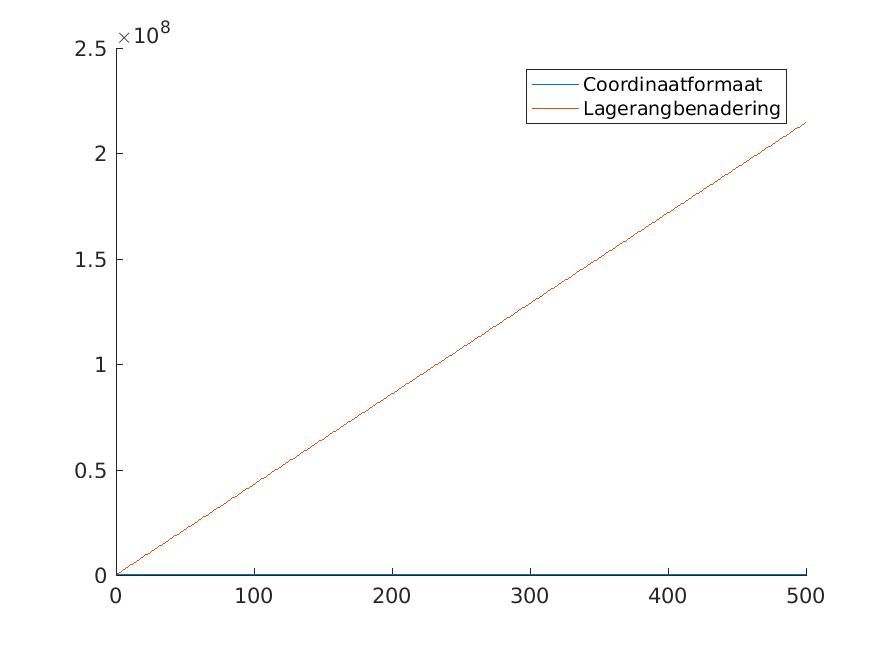
\includegraphics[width=0.7\linewidth]{../ex2}
		\caption{}
		\label{fig:ex2}
	\end{figure}

    De twee functies snijden nooit en ik moet de berekening eens checken.

	\subsubsection{Opdracht 3}
    \begin{quote}
        Bewijs dat \(\sigma_j\) de \(j^de\) grootste singuliere waarde van A is en dat
        \[ A - E_k = \sum\limits_{j=1}^{k} \sigma_j \textbf{u}_j \textbf{v}_j^T \]
        de rang-k (met \( k \leq r \)) afgeknotte singulierewaardeontbinding van A is.
    \end{quote}

	\subsubsection{Opdracht 4}
    \begin{quote}
        Stel dat we de stappen 4–6 van algoritme 1 slechts eenmaal zouden uitvoeren.
        Kan men dit algoritme dan toepassen op een 240 000×33 000 matrix met 22 miljoen niet-nulwaarden
        (i.e., de volledige MovieLens databank) op een laptop met 8GB werkgeheugen en 32GB swap geheugen? Waarom wel of niet?
    \end{quote}

    Dit is enkel mogelijk als ijle matrices worden gebruikt. Bij gebruik van volle matrices is er te veel geheugenruimte nodig.

	Output van de code (te vinden in \ref{appendix:ex4}):
\begin{lstlisting}
Totaal bruikbaar geheugen: 40GB
Nodig geheugen met volle matrices: 118.02GB
Nodig geheugen als het ijlhijdspatroon behouden kan worden: 0.66GB
\end{lstlisting}

	\subsubsection{Opdracht 5}
    \begin{quote}
        function [X] = SN\_sparseModel(Uk,sk,Vk,A). \\
        De geheugencomplexiteit van je algoritme in functie van m, n, r en \(\zeta\) mag hoogstens \(\mathcal{O}(\zeta)\) bedragen
        - je mag hierbij wel veronderstellen dat \( max\{m, n\} \leq \zeta \). Hoe heb je deze doelstelling bereikt?
    \end{quote}

	\subsubsection{Opdracht 6}
    \begin{quote}
        function [s] = SN\_optimalCoefficients(Uk,Vk,A)
        De geheugencomplexiteit van je algoritme in functie van m, n, k en ζ mag hoogstens \(\mathcal{O}(k\zeta)\) bedragen
        - je mag hierbij wel veronderstellen dat \( max\{m, n\} \leq \zeta \). Hoe heb je deze doelstelling bereikt?
    \end{quote}

	\subsubsection{Opdracht 8}
    \begin{quote}
        Hoeveel bedragen de 3 laagste gemiddelde beoordelingen? Hoeveel gebruikers gaven exact 5 als gemiddelde score?
    \end{quote}

	\subsubsection{Opdracht 10}
    \begin{quote}
        Hoeveel bedraagt de RMSE tussen T en de ijle matrix \( P_{\Omega}(\boldsymbol{\mu} \boldsymbol{1}^T ) \)?
    \end{quote}

	\subsubsection{Opdracht 11}
    \begin{quote}
        Pas SN\_rank1MatrixPursuit toe op de gekende beoordelingenmatrix R, waarbij je r = 30 als gewenste rang kiest en de testdata T
        als derde argument kiest. Maak een duidelijke figuur van de evolutie van de RMSE van algoritme 2. Neem de figuur op in het verslag.
    \end{quote}

	\subsubsection{Opdracht 12}
    \begin{quote}
        Bereken [U20,s20,V20,~] = SN\_rank1MatrixPursuit(R,20,T). Wat zijn de waarden van de vector s20, afgerond tot 2 cijfers na de komma?
    \end{quote}

	\subsubsection{Opdracht 14}
    \begin{quote}
        function [movieIDs, score] = SN\_predictedBestMovies(Uk,sk,Vk)
        De geheugencomplexiteit van je algoritme in functie van m, n en k mag hoogstens \(\mathcal{O}(max\{m, n\})\) bedragen.
        Hoe heb je deze doelstelling bereikt?
    \end{quote}

	\subsubsection{Opdracht 15}
    \begin{quote}
        Bereken met behulp van de functies uit de twee voorgaande opgaves de 25 films met de hoogste gemiddelde beoordelingen
        (op basis van de gekende beoordelingenmatrix R) en de 25 films met de hoogste gemiddelde voorspelde beoordelingen. \\
        Welke lijst van films vind je het meest realistisch? Motiveer je keuze. Onderzoek in het bijzonder het aantal gekende
        beoordelingen in de trainingsdata R van de films in de twee lijsten en betrek deze informatie in je motivering.
    \end{quote}


	\subsection{Clustering}

	\subsubsection{Opdracht 16}
    \begin{quote}
        De geheugencomplexiteit van je algoritme in functie van m, n en k mag hoogstens \(\mathcal{O}(k^2 + n^2)\) bedragen.
        Hoe heb je deze doelstelling bereikt?
    \end{quote}

	\subsubsection{Opdracht 18}
    \begin{quote}
        Welke n films zijn het sterkst positief gecorreleerd met de film met volgnummer k, voor volgende waarden van n en k?
        Zijn deze resultaten realistisch? Motiveer. Zijn er gelijkenissen met de aanbevelingen van andere aanbevelingssystemen,
        zoals bijvoorbeeld IMDB.com, MovieLens, Amazon.com of Netflix?
    \end{quote}

	\subsubsection{Opdracht 19}
    \begin{quote}
        Bewijs dat de correlatiematrix C in vergelijking (8) hoogstens rang r + 1 heeft wanneer de voorspelde beoordelingenmatrix
        A exact rang r heeft.
    \end{quote}


\section{Evaluatie}

	\subsection{Opdracht 1}
		\begin{quote}
			Hoeveel tijd heb je gespendeerd aan het oplossen van de opdrachten?
			Hoeveel tijd heb je gespendeerd aan het schrijven van het verslag?
		\end{quote}
        Ik heb ongeveer 23 uur gespendeerd aan het oplossen van de opdrachten en ongeveer 4 uur aan het schrijven van het verslag.

	\subsection{Opdracht 2}
		\begin{quote}
			In de loop van deze opdracht hebben we allerhande veronderstellingen gemaakt om ons nieuw aanbevelingssysteem
             op te stellen. Wat zijn je bedenkingen hierbij? Vind je de resultaten realistisch? Zou je het ontwikkelde
             aanbevelingssysteem durven toevoegen aan de lijst van aanbevelingssystemen van MovieLens?
		\end{quote}



	\subsection{Opdracht 3}
		\begin{quote}
			Welke bedenkingen heb je bij dit practicum? Was de opdracht (veel) te gemakkelijk, (veel) te moeilijk of
			van een gepaste moeilijkheidsgraad? Wat zou je zelf anders aangepakt hebben?  Was de terminologie voldoende duidelijk?
		\end{quote}




\onecolumn
\appendix
\appendixpage
\addappheadtotoc

\section{Code}
	\subsection{Opdracht 2}
		\lstinputlisting[style=Matlab-editor, basicstyle = \scriptsize]{../ex2.m}
	\subsection{Opdracht 4}
    \label{appendix:ex4}
		\lstinputlisting[style=Matlab-editor, basicstyle = \scriptsize]{../ex4.m}
    \subsection{Opdracht 5}
        \lstinputlisting[style=Matlab-editor, basicstyle = \scriptsize]{../ex5.m}
    \subsection{Opdracht 6}
        \lstinputlisting[style=Matlab-editor, basicstyle = \scriptsize]{../ex6.m}
    \subsection{Opdracht 8}
        \lstinputlisting[style=Matlab-editor, basicstyle = \scriptsize]{../ex8.m}
	\subsection{Opdracht 10}
		\lstinputlisting[style=Matlab-editor, basicstyle = \scriptsize]{../ex10.m}
	\subsection{Opdracht 11}
		\lstinputlisting[style=Matlab-editor, basicstyle = \scriptsize]{../ex11.m}
	\subsection{Opdracht 12}
		\lstinputlisting[style=Matlab-editor, basicstyle = \scriptsize]{../ex12.m}
	\subsection{Opdracht 15}
		\lstinputlisting[style=Matlab-editor, basicstyle = \scriptsize]{../ex15.m}
	\subsection{Opdracht 18}
		\lstinputlisting[style=Matlab-editor, basicstyle = \scriptsize]{../ex18.m}

    \subsection{r0679689\_sparseModel.m}
		\lstinputlisting[style=Matlab-editor, basicstyle = \scriptsize]{../r0679689_sparseModel.m}
    \subsection{r0679689\_optimalCoefficients.m}
		\lstinputlisting[style=Matlab-editor, basicstyle = \scriptsize]{../r0679689_optimalCoefficients.m}
	\subsection{r0679689\_userMeans}
		\lstinputlisting[style=Matlab-editor, basicstyle = \scriptsize]{../r0679689_userMeans.m}
    \subsection{r0679689\_RMSE}
		\lstinputlisting[style=Matlab-editor, basicstyle = \scriptsize]{../r0679689_RMSE.m}
    \subsection{r0679689\_rank1MatrixPursuit.m}
		\lstinputlisting[style=Matlab-editor, basicstyle = \scriptsize]{../r0679689_rank1MatrixPursuit.m}
    \subsection{r0679689\_actualBestMovies.m}
		\lstinputlisting[style=Matlab-editor, basicstyle = \scriptsize]{../r0679689_actualBestMovies.m}
    \subsection{r0679689\_predictedBestMovies.m}
		\lstinputlisting[style=Matlab-editor, basicstyle = \scriptsize]{../r0679689_predictedBestMovies.m}
    \subsection{r0679689\_correlationMatrix.m}
		\lstinputlisting[style=Matlab-editor, basicstyle = \scriptsize]{../r0679689_correlationMatrix.m}
    \subsection{r0679689\_similarMovies.m}
		\lstinputlisting[style=Matlab-editor, basicstyle = \scriptsize]{../r0679689_similarMovies.m}
\end{document}
